\documentclass[PhD-Yoann-Dupont.tex]{subfiles}
\begin{document}

Le participant ayant remporté la première place \citep{dinarelli2012} a proposé une cascade de deux modèles. Le premier, un CRF, permet d'annoter les feuilles des arbres. Le second, une grammaire lexicalisée probabiliste (PCFG) permet de retrouver le reste de la structure arborée. Cet enchainement de modèles est illustré dans la figure \ref{fig:dinarelli-cascade}.

%\begin{figure}[ht!]
%\centering
%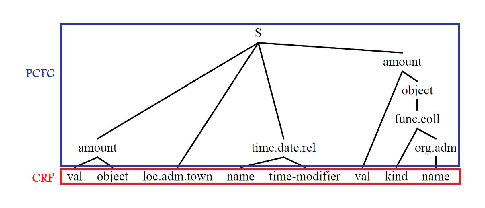
\includegraphics[scale=1.5]{images/models-cascade/crf-pcfg-cascade}
%\caption{illustration de la cascade CRF+PCFG proposée par \citet{dinarelli2012} sur une phrase.}
%\label{fig:dinarelli-cascade}
%\end{figure}
\begin{figure}[ht!]
\centering
\scriptsize
\begin{forest}
    for tree={
        l+=0.5cm,
    }
    [\textbf{S}
        [\textbf{func.ind},name=A
            [\textbf{O},l*=2 [notre]]
            [\textbf{kind},l*=2 [président]]
            [\textbf{O},l*=2 [{,}]]
            [\textbf{pers.ind}
                [\textbf{qualifier} [M.]]
                [\textbf{name.first} [Nicolas]]
                [\textbf{name.last} [Sarkozy]]
            ]
        ]
    ]
    \draw[blue] (-3,0.375) -- (5.375,0.375) -- (5.375,-2.75) -- (-3,-2.75) -- (-3,0.375);
    \node[blue,align=left] at (-3.75,-1.125) {\textbf{PCFG}};
    \draw[red] (-3,-3.6) -- (5.375,-3.6) -- (5.375,-4) -- (-3,-4) -- (-3,-3.6);
    \node[red,align=left] at (-3.75,-3.8) {\textbf{CRF}};
\end{forest}
\caption{illustration de la cascade CRF+PCFG proposée par \citet{dinarelli2012} sur une phrase.}
\label{fig:dinarelli-cascade}
\end{figure}

Une PCFG est définie formellement comme un quintuplet $G = (M, T, R, S, Q)$ où :
\begin{itemize}
    \item M est l'alphabet des symboles non-terminaux,
    \item T est l'alphabet des symboles terminaux,
    \item R est l'ensemble des règles de production,
    \item S est l'axiome V,
    \item Q est l'ensemble des probabilités des règles de production.
\end{itemize}

~\\
Une règle $r \in R$ se note $\alpha \rightarrow \beta$ pour signifier "$\alpha$ produit $\beta$", où $\alpha$ et $\beta$ sont appelés respectivement le producteur et le produit de la règle $r$.

Soient $\alpha \in M$ un non-terminal, $N_{\alpha}$ l'ensemble règles de production de $R$ telles que $N_{\alpha}(i) = \alpha \rightarrow \beta_(i)$, de taille $T$, avec $N_{\alpha} \subset R$. Les PCFG vérifient la propriété suivante :

\begin{equation}
\sum_{i=1}^{T} q(N_{\alpha}(i)) = \sum_{i=1}^{T} q(\alpha \rightarrow \beta_{i})) = 1.0
\end{equation}

Autrement dit:

\begin{equation}
q(\alpha \rightarrow \beta) = p(\beta|\alpha) = \frac{p(\alpha,\beta)}{p(\alpha)}
\end{equation}

Une PCFG peut être dérivée d'un corpus arboré (ensemble d'exemples). Si nous reprenons la phrase de la figure \ref{fig:address-tree}. Nous pouvons inférer la PCFG suivante :
\begin{itemize}
\item M $\leftarrow$ \{numéro-rue, type-voie, nom-rue, code-postal, ville, personne, prénom, nom\}
\item T $\leftarrow$ \{1, rue, Maurice, Arnoux, 92120, Montrouge\}
\item R $\leftarrow$
    \begin{itemize}
    \item adresse $\rightarrow$ numéro-rue, type-voie, nom-rue, code-postal, ville
    \item nom-rue $\rightarrow$ personne
    \item personne $\rightarrow$ prénom, nom
    \item numéro-rue $\rightarrow$ 1
    \item type-voie $\rightarrow$ rue
    \item prénom $\rightarrow$ Maurice
    \item nom $\rightarrow$ Arnoux
    \item code-postal $\rightarrow$ 92120
    \item ville $\rightarrow$ Montrouge
    \end{itemize}
\item S $\leftarrow$ adresse
\item Q $\leftarrow$ \textcolor{green!60!black}{\textit{dans cet exemple, toutes les règles ont une probabilité de 1.}}
\end{itemize}

Lorsqu'une grammaire est dérivée d'un corpus, les probabilités pour les règles sont déduites à partir de comptages d'occurrences à l'échelle du corpus. Ainsi, la probabilité d'une règle $\alpha\ \rightarrow\ \beta$, $q(\alpha\ \rightarrow\ \beta)$, se définit comme suit :

\begin{equation}
q(\alpha\ \rightarrow\ \beta) = \frac{count(\alpha\ \rightarrow\ \beta)}{count(\alpha)}
\end{equation}

Où count($\alpha\ \rightarrow\ \beta$) est le nombre d'occurrences de la règle $\alpha\ \rightarrow\ \beta$ dans le corpus et count($\alpha$) le nombre d'occurrences du non-terminal $\alpha$ dans le corpus.

L'algorithme classiquement utilisé pour effectuer le parsing d'une séquence à l'aide d'une grammaire est l'algorithme CYK (Cocke, Younger and Kasami) \citep{hays1962automatic,kasami1965efficient,younger1967recognition}\footnote{Hays est la référence la plus ancienne attribuant la parenté de l'algorithme à Cocke. Cela est également indiqué par \citet{jacobs1990parsing}, page 576.}. Cet algorithme attend une grammaire en forme normale de Chomsky (CNF), qui restreint les règles de R à avoir une des deux formes suivantes :

\begin{itemize}
    \item NonTerminal $\rightarrow$ NonTerminal1 \ NonTerminal2
    \item NonTerminal $\rightarrow$ terminal
\end{itemize}

Il a par la suite été étendu pour notamment gérer les règles dites unaires, qui ont la forme "NonTerminal1 $\rightarrow$ NonTerminal2", la grammaire étant alors dite seulement binarisée. Ces règles sont particulièrement utiles dans le cadre des entités nommées structurées, où il existe de nombreuses règles unaires (avec un schéma d'annotation Quaero au moins). En effet, les entités nommées de type organisation ou lieu ont typiquement un composant de type nom de même étendue. La grammaire présentée précédemment n'est pas binarisée : son axiome a une partie droite comprenant 5 non-terminaux. La binarisation se fait alors en créant de nouvelles règles à la grammaire. La binarisation de S donnerait les règles suivantes :
\begin{itemize}
    \item S $\rightarrow$ numéro-rue, $X_{1}$
    \item $X_{1}$ $\rightarrow$ type-voie, $X_{2}$
    \item $X_{2}$ $\rightarrow$ nom-rue, $X_{3}$
    \item $X_{3}$ $\rightarrow$ code-postal, ville
\end{itemize}

Où $X_{n}$ sont des règles absentes de la grammaire de base qui pourront alors être supprimées après l'application de CYK afin d'obtenir la structure véritable de l'arbre d'analyse.

L'un des inconvénients de cette approche est que les entités nommées ne forment pas un arbre de constituants syntaxiques, de nombreux n\oe uds dans ce dernier étant alors "vides", un symbole spécial leur étant attribué. Nous noterons le symbole de n\o eud vide par "O", comme illusté dans la figure \ref{fig:dinarelli-cascade}. Ce système ayant servi de baseline pour ses expériences, nous l'appelerons donc \textit{tree-baseline}. \citet{dinarelli2012} a alors enrichi les arbres avec plus ou moins d'information, afin de fournir aux systèmes par apprentissage plus de contexte. En plus du système \textit{tree-baseline}, plusieurs variantes ont donc été proposées. Nous nous concentrerons sur les variantes \textit{parent-context}, utilisée durant la campagne Quaero, et \textit{parent-node-filler}, dont les résultats sont meilleurs mais n'ont été obtenus qu'après la campagne. \textit{Parent-context} ajoute à chaque n\oe ud vide l'information du parent dans l'arbre d'analyse et est illustrée dans la figure \ref{fig:parent-context}. \textit{Parent-node-filler} distingue les éléments "O" si ces derniers sont présents dans une entité en leur attribuant une étiquette particulière et ajoute aux n\oe uds ayant une annotation non-vide l'information du parent. Cette variante est illustrée dans la figure \ref{fig:parent-node-filler}.
    
\begin{figure}[ht!]
\centering
\scriptsize
\begin{forest}
  for tree={l+=0.5cm} % increase level distance
  [\textcolor{blue}{\textbf{func.ind}}
    [\textcolor{red}{\textbf{func.ind@O}} [notre]]
    [\textcolor{red}{\textbf{kind}} [président]]
    [\textcolor{red}{\textbf{func.ind@O}} [{,}]]
    [\textcolor{blue}{\textbf{pers.ind}}
        [\textcolor{red}{\textbf{qualifier}} [M.]]
        [\textcolor{red}{\textbf{name.first}} [Nicolas]]
        [\textcolor{red}{\textbf{name.last}} [Sarkozy]]
    ]
  ]
\end{forest}
\caption{La représentaion \textit{parent-context} utilisée pendant la campagne.}
\label{fig:parent-context}
\end{figure}
    
\begin{figure}[ht!]
\centering
\scriptsize
\begin{forest}
  for tree={l+=0.5cm} % increase level distance
  [\textcolor{blue}{\textbf{func.ind}}
    [\textcolor{red}{\textbf{ne-filler}} [notre]]
    [\textcolor{red}{\textbf{func.ind@kind}} [président]]
    [\textcolor{red}{\textbf{ne-filer}} [{,}]]
    [\textcolor{blue}{\textbf{func.ind@pers.ind}}
        [\textcolor{red}{\textbf{pers.ind@qualifier}} [M.]]
        [\textcolor{red}{\textbf{pers.ind@name.first}} [Nicolas]]
        [\textcolor{red}{\textbf{pers.ind@name.last}} [Sarkozy]]
    ]
  ]
\end{forest}
\caption{La représentaion \textit{parent-node-filler} ayant donné les meilleurs résultats après la campagne.}
\label{fig:parent-node-filler}
\end{figure}
    
    Les résultats des différentes variantes sont donnés dans le tableau \ref{tab:md-quaero-results}. Il existe deux inconvénients à cette approche. Le premier, mineur, est que les entités nommées arborées ne donnent qu'une analyse partielle de la phrase, où les algorithmes classiques attendent une analyse complète. Les arbres doivent alors être adaptés en incluant de nombreux n\oe uds vides, qui seront supprimés par la suite. Ces modèles ont également l'inconvénient d'avoir une grande complexité algorithmique, cette dernière étant en général cubique pour une PCFG. Pour ces raisons, nous avons voulu essayer une approche algorithmiquement plus simple, se basant sur des cascades de modèles linéaires.
    
    \begin{table}
    \centering
    \begin{tabular}{|c|c|}
    \hline
    Model & SER \\
    \hline
    baseline & 33.4 \\
    parent-context & 33.3 \\
    parent-node-filler & 30.2 \\
    \hline
    \end{tabular}
    \caption{les résultats obtenus sur le Quaero par \citet{dinarelli2012} selon les informations ajoutées.}
    \label{tab:md-quaero-results}
    \end{table}

\end{document}